\chapter{Matrix-Vector Product}

When we take the product of the matrix and the vector, 
it will result in a vector. The product is a contraction 
operation, which means that the matrix's dimension reduced from two to one.
To apply the contraction, then the length of one of the matrix dimensions 
must be the same as the vector's length.

Let the $A$ be the matrix with dimensions $m$ and $n$, 
and the length of the vector $x$ be $n$.

The resultant vector $y$ will have the dimension $m$.

\vspace*{0.5 cm}
$
A = 
\begin{bmatrix}
    a_{00}  & a_{01}    & \dots     & a_{0n}\\
    a_{10}  & a_{11}    & \dots     & a_{1n}\\
    \vdots  & \vdots    & \ddots    & \vdots\\
    a_{m0}  & a_{m1}    & \dots     & a_{mn}\\
\end{bmatrix}
, x =
\begin{bmatrix}
    x_0\\
    x_1\\
    \vdots\\
    x_n\\
\end{bmatrix}
$

\begin{equation}
    y = Ax + y
    \label{eq:mtv}
\end{equation}

$
Av = 
\begin{bmatrix}
    a_{00}  & a_{01}    & \dots     & a_{0n}\\
    a_{10}  & a_{11}    & \dots     & a_{1n}\\
    \vdots  & \vdots    & \ddots    & \vdots\\
    a_{m0}  & a_{m1}    & \dots     & a_{mn}\\
\end{bmatrix}
\begin{bmatrix}
    x_0\\
    x_1\\
    \vdots\\
    x_n\\
\end{bmatrix}
=
\begin{bmatrix}
    \sum_{i=0}^na_{0i}x_i\\
    \sum_{i=0}^na_{1i}x_i\\
    \vdots\\
    \sum_{i=0}^na_{mi}x_i\\
\end{bmatrix}
$

\vspace*{0.5 cm}
The vector times matrix can calculated by taking the transpose on the both sides.
\begin{align*}
    y^T &= (Ax + y)^T\\
    y^T &= (Ax)^T + y^T\\
    y^T &= x^TA^T + y^T\\
\end{align*}

The column-major and row-major layout for the vector in the memory 
is non-distinguishable. Hence, we can use this fact and we get $x = x^T$.
If $A$ is the column-major layout then $A^T$ is the row-major layout and vice-versa.

\begin{equation}
    y = xA^T + y
    \label{eq:vtm}
\end{equation}

\clearpage
\section{Calculating Number of Operations}

Using equation \ref{eq:mtv} or \ref{eq:vtm}, we fill the below table

\begin{table}[ht]
    \centering
    \begin{tabular}{|c|c|}
        \hline
        \textbf{Name} & \textbf{Number} \\
        \hline
        Multiplication & $m$ or $n$\\
        \hline
        Addition & $m-1$ or $n-1$ \\
        \hline
    \end{tabular}
\end{table}

Total Number of Operations $=$ (Number of Multiplication $+$ Number of Addition) $\times
\begin{cases}
    n \\
    m
\end{cases}
$

Total Number of Operations $= 
\begin{cases}
    n \times (m + m - 1)\\
    m  \times (n + n - 1)
\end{cases}
$

Total Number of Operations $= 
\begin{cases}
    n \times (2m - 1)\\
    m  \times (2n - 1)
\end{cases}
$

\section{Algorithm}
The matrix-vector product has two different algorithms: 
Column-Major and Row-Major. We need to handle two different 
layouts differently. 
The Row-Major has the most straightforward algorithm because 
the row elements lay contiguously in the memory, which improves 
the cache locality compared against Column-Major, where the row 
elements placed with a specific stride and hinder the cache locality.

\subsection{Column-Major}

\begin{algorithm}[H]
    \SetAlgoLined
    \SetKwFunction{SIMDFn}{$simd\_loop_N$}
    \SetKwProg{Fn}{Function}{:}{end}

    \tcp{$c$ is the pointer to the output vector}
    \tcp{$a$ is the pointer to the input matrix}
    \tcp{$b$ is the pointer to the input vector}
    \tcp{$block$ is the block of the output vector}
    \tcp{$w$ is the leading dimension of the matrix}
    \tcp{$simd\_loop_N$ is a function where N signifies the amount of the unrolling done}
    \Fn{\SIMDFn($c$, $a$, $b$, $block$, $w$)}{
        \openmp{simd}
        \For{\assign{i}{0} \KwTo $block$ \KwBy $1$}{
            $    
            \begin{matrix}
                c[i] \gets c[i] +  A[i + w * 0] * b[0];\\
                c[i] \gets c[i] +  A[i + w * 1] * b[1];\\
                \vdots\\
                c[i] \gets c[i] +  A[i + w * N] * b[N];\\
            \end{matrix}
            $
        }
    }
    \caption{Matrix-Vector Product SIMD Function}
\end{algorithm}

\begin{algorithm}[H]
    \SetAlgoLined
    \SetKwFunction{SIMDFn}{$main\_loop_N$}
    \SetKwProg{Fn}{Function}{:}{end}

    \tcp{$c$ is the pointer to the output vector}
    \tcp{$a$ is the pointer to the input matrix}
    \tcp{$b$ is the pointer to the input vector}
    \tcp{$n_a$ is the size of the column of the matrix $a$}
    \tcp{$w_a$ is the leading dimension of the matrix $a$}
    \tcp{$n_b$ is the size of the vector $b$}
    \tcp{$block$ is the block of the output vector}
    \tcp{$main\_loop_N$ is a function where N signifies the amount of the unrolling done}
    \Fn{\SIMDFn($c$, $a$, $n_a$, $w_a$, $b$, $n_b$, $block$)}{
        \If{$n_b == 0$}{
            \KwRet{};
        }
        \assignln{ai}{a}
        \assignln{bi}{b}
        \assignln{ci}{c}
        \openmp{for schedule(dynamic)}
        \For{\assign{i}{0} \KwTo $n_a$ \KwBy $block$}{
            \assignln{aj}{ai + i}
            \assignln{bj}{bi}
            \assignln{cj}{ci + i}
            \assignln{ib}{min(block,na-i)}
            \For{\assign{j}{0} \KwTo $n_b$ \KwBy $1$}{
                \assignln{ak}{a + j \times N \times wa}
                \assignln{bk}{bk + j \times N}
                \assignln{ck}{cj}
                $simd\_loop_N(ck,ak,bk,ib,w_a)$
            }
        }
    }
    \caption{Matrix-Vector Product Loop}
\end{algorithm}

\begin{algorithm}[H]
    \SetAlgoLined
    \KwIn{$c$, $a$, $n_a$, $w_a$, $b$, $n_b$, $max\_threads$}
    \tcp{$c$ is the pointer to the output vector}
    \tcp{$a$ and $b$ are pointer to the matrix}
    \tcp{$b$ are pointer to the vector}
    \tcp{$n_a$ is the size of the column of the matrix $a$}
    \tcp{$w_a$ is the leading dimension of the matrix $a$}
    \tcp{$n_b$ is the size of the vector $b$}
    \tcp{$max\_threads$ is the user provided thread count}

    \Begin{
        $omp\_set\_num\_threads(max\_threads)$

        \assignln{number\_el\_L_1}{\lfloor \frac{S_{L_1}}{S_{data}} \rfloor}
        \assignln{half\_block}{\lfloor \frac{number\_el\_L_1}{2} \rfloor}
        \assignln{max\_size}{max(na,nb)}
        \assign{small\_block}{2^{\lfloor \frac{k}{2} \rfloor}}
        \tcp{Where $2^k$ is a power of two representation of $number\_el\_L_1$}
        
        \assignln{k\_factor}{nearest\_power\_of\_2(\frac{number\_el\_L_1}{\log_2{small\_block}})}
        \assignln{block_2}{max(1, \frac{small\_size}{2^{\lfloor \frac{max\_size}{k\_factor} \rfloor}})}

        \If{$n_a > number\_el\_L_1$}{
            \assignln{block_1}{half\_block}
            }
        \Else{
            \assignln{block_1}{small\_block}
        }

        \assignln{n_{itr}}{\lfloor \frac{n_b}{block_2} \rfloor}
        \assign{n_{rem}}{n_b - (block_2 \times \lfloor \frac{n_b}{block_2} \rfloor)}
        \tcp{This equation gives the remainder}

        \openmp{parallel}
        \Begin{
            $main\_loop_1(c,a,w_a,n_a,b,n_{rem},block_1)$
            
            \assignln{at}{a + w_a \times n_{rem}}
            \assignln{bt}{b + n_{rem}}
            $main\_loop_{block_2}(c,at,w_a,n_a,bt,n_{iter},block_1)$
        }

    }

    \caption{Col-Major Matrix-Vector Product}
\end{algorithm}

The Column-Major product is quite tricky and complicated if 
we cannot control the instruction set. 
The row elements are $x$ strides away from each other and 
paralyse the cache predictor or cache locality. 
The cache predictor brings the cache line size elements 
from memory, which are place contiguously. 
Each element in the result vector is the product of the 
matrix's row vector and the whole vector. 

For OpenMP to do its magic, we need to fill the $L_1$ cache with 
the result vector block, block of the input vector's matrix and block. 
We divide the load through the threads, where each thread has 
its private cache, and they calculate a small block of the 
result vector without hindering the other vectors. 
The result vector calculation is done by dividing it into 
smaller chunk or block and handing over the block to each thread, 
which removes the dependency within the different blocks and 
eradicates the data races and synchronization. 
The loop which manages the block for the result 
vectors must be multithreaded, and each thread needs to fill 
the $L_1$ cache with the output vector and a column vector of the matrix 
as large as it can so that the registers can fetch the blocks as fast 
as possible from the cache rather than fetching from memory, which adds 
an overhead to the performance. To fit the output vector, the matrix and the vector, 
we previously discussed fact and the \ref{fig:mtv_col_block_diagram} 
for the variable convention; we derive the following equation.

\begin{equation}
    S_{L_1} = S_{data}(m_cn_c + m_c + n_c)
    \label{eq:mtv_col_block} 
\end{equation}

\begin{figure}[htb]
    \centering
    \caption{Column-Major Matrix-Vector Block Diagram}
    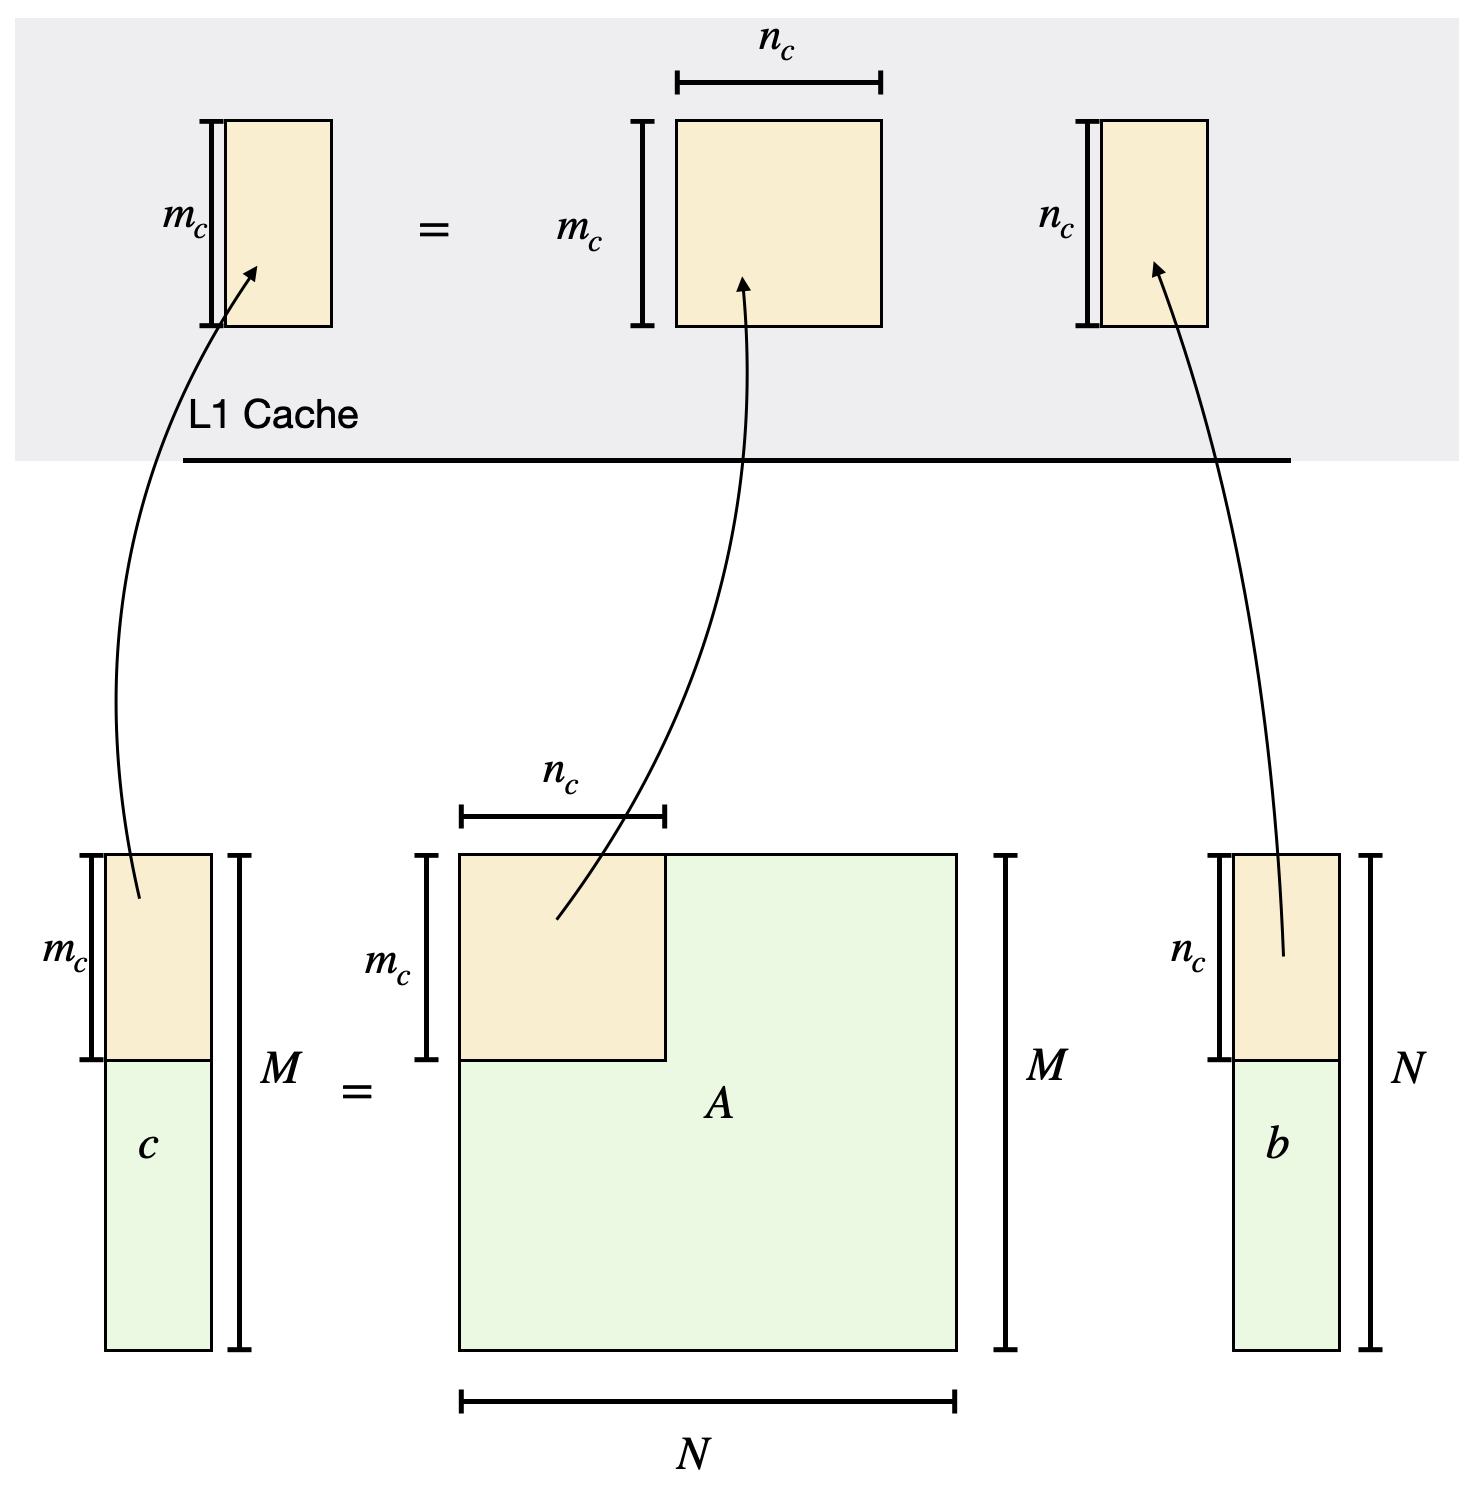
\includegraphics[width=10cm]{../assets/mtv/col_major/block_diagram.png} %
    \label{fig:mtv_col_block_diagram}
\end{figure}


For the small length of the result vector, which is less than the L1 
cache size, to maximize the block in the L1 cache, the row block and 
column block must be identical, $m_c = n_c$, which makes the matrix a square matrix.

Let $m_c = n_c = B_{small}$
\begin{align*}
    S_{L_1} &= S_{data}(m_cn_c + m_c + n_c)\\
    S_{L_1} &= S_{data}(B_{small} \times B_{small} + B_{small} + B_{small})\\
    S_{L_1} &= S_{data}(B_{small}^2 + 2B_{small})\\
\end{align*}

\begin{equation}
    B_{small}^2 + 2B_{small} = \frac{S_{L_1}}{S_{data}}
    \label{eq:mtv_col_small_block} 
\end{equation}

$B_{small}^2$ is much larger than the $2B_{small}$ in \ref{eq:mtv_col_small_block}, so we can ignore the smaller term.

\[B_{small}^2 < \frac{S_{L_1}}{S_{data}}\]

We can represent $\frac{S_{L_1}}{S_{data}}$ in form of power of two because 
we know both $S_{L_1}$ and $S_{data}$ are power of two. Therefore, the division must 
produce a power of two. Let the exponent of two be $k$, which gives us

\begin{align*}
    B_{small}^2 &< 2^k\\
    B_{small} &< 2^{\frac{k}{2} }
\end{align*}

Here, $k$ can be both even or odd. We will have a fractional value if $k$ is odd, 
and we cannot have a fractional value because we have no control over the registers, 
and registers are always discrete, which is a multiple of a power of two. 
We try to maximize the register use, and if the value is fractional, 
it will not fill the registers fully, and it is a wastage of processing power. 
There might be a case when the register has only one element, and subsequent 
iteration will have to fill the register with more elements; we could have filled 
the register with the following elements and had processed more elements rather 
than waiting for subsequent iteration, which is a wastage of cycles.

\begin{align*}
    2^{\lfloor \frac{k}{2} \rfloor} &\leq 2^{\frac{k}{2}} \leq 2^{\lceil \frac{k}{2} \rceil}\\
    \lfloor \frac{k}{2} \rfloor &\leq \frac{k}{2} \leq \lceil \frac{k}{2} \rceil\\
\end{align*}

using this relation and taking the lower bound, we have

\begin{equation}
    B_{small} \leq 2^{\lfloor \frac{k}{2} \rfloor}
    \label{eq:mtv_col_small_block_simplified} 
\end{equation}

The eqauation \ref{eq:mtv_col_small_block_simplified} is only valid if the length of the output
vector is less than the $L_1$ cache.

$B_{small}$ is the lower bound, so now, we need to find the upper bound. 
To find the upper bound, we will use the fact that each thread has its 
private cache, an $L_1$ cache. Using the equation \ref{eq:mtv_col_block}, 
we can maximize the output vector's block by putting an 
input vector element into the register, making the block of 
the input vector one, $m_c$ by putting an input vector element into the 
register, which makes the block of the input vector one, $n_c = 1$. We do not need $n_c$
in the $L_1$ cache, so we remove it from the equation \ref{eq:mtv_col_block}.

\begin{align*}
    S_{L_1} &= S_{data}(m_cn_c + m_c)\\
    S_{L_1} &= S_{data}(m_c + m_c)\\
    S_{L_1} &= S_{data}(2m_c)\\
    m_c &= \frac{S_{L_1}}{2S_{data}}\\
\end{align*}

When $M < \frac{S_{L_1}}{S_{data}}$ then $m_c = B_{small}$, otherwise, $m_c = \frac{S_{L_1}}{2S_{data}}$.

\vspace*{0.5 cm}
Now, we need to find block $n_c$, where $n_c$ is an unrolling factor. 
The unrolling factor helps to bring the block of column vectors 
in the cache, and the block is the size of the cache line. 
If the cache line size and $m_c$ are of the same size, then the 
cache misses minimized. We found that $n_c$ is a decreasing value 
through experiments and depends on the maximum dimension, 
where it reaches the minimum value of one when the maximum dimension 
is equal to or exceeds the $L_1$ cache size.

We see this behaviour due to the cache misses as the dimension 
increase in size, the block $n_c$ starts to replace the block of 
output vector $m_c$ using the LRU policy, so on the subsequent iteration, 
the replaced block of the output $m_c$ again needs to bring back to the $L_1$ cache.

Let $cm_X$ be the cache miss where $X$ is the size of the block.
For the large block of $n_c$ and the large dimension.

$Total\ Cache\ Misses = $ cache miss for bringing the block $m_c$ of the output into the cache $+$
cache miss for bringing the block $m_c \times n_c$ of the matrix $A$ into the cache $+$
cache miss for bringing the block $m_c - Size(Register)$ of the output into the cache back which was
replaced due to eviction + cache miss for bringing the block $n_c$ of the input into the cache.

\[Total\ Cache\ Misses = cm_{m_c} + cm_{m_cn_c} + cm_{m_c - Size(Register)} + cm_{n_c}\]

If the $n_c = 1$ for the large length then $cm_{n_c} = 0$ because it will reside inside the register 
and there is no cache eviction. Therefore, $cm_{m_c - Size(Register)} = 0$, so we have
\begin{align*}
    Total\ Cache\ Misses &= cm_{m_c} + cm_{m_c}\\
    Total\ Cache\ Misses &= 2cm_{m_c}\\
\end{align*}

Using this fact, we can deduce
\[1 \leq n_c \leq B_{small}\]

Since $n_c$ is a decreasing value and we decrease $n_c$ by the power of two 
because we need to use the register efficiently. Let $S_{max}$ be the maximum dimension 
of the matrix.

\begin{figure}[htb]
    \centering
    \caption{Input Vector Block Divison Diagram}
    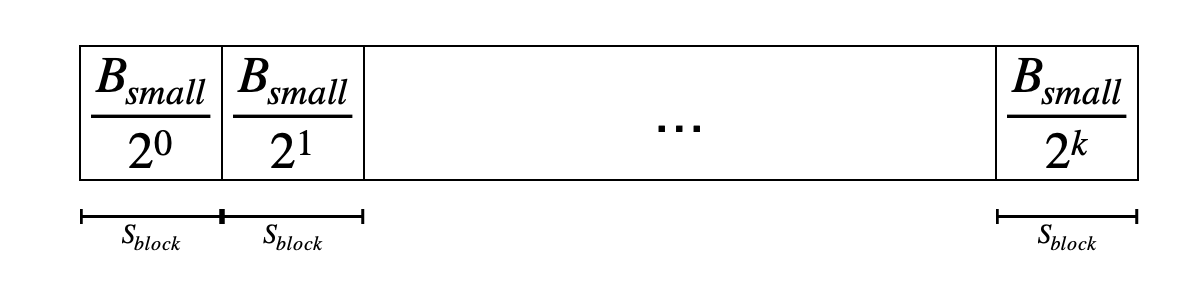
\includegraphics[width=15cm]{../assets/mtv/col_major/input_block_diagram.png} %
\end{figure}

Using the previously derived facts, we know $\frac{B_{small}}{2^k} = 1$ 
when $\frac{S_{L_1}}{S_{data}} \leq S_{max}$

\[\frac{B_{small}}{2^k} = 1\]
\[B_{small} = 2^k\]
\[k = \log_2{B_{small}}\]
\[kS_{block} = \frac{S_{L_1}}{S_{data}}\]
\[S_{block} = \frac{S_{L_1}}{kS_{data}}\]

\begin{equation}
    S_{block} = \frac{S_{L_1}}{S_{data} \log_2{B_{small}}}
\end{equation}

If the $S_{block}$ is not the power of two then get the nearest power of two.
\[2^q \leq S_{block} \leq 2^{q+1}\]

Therefore,
\begin{equation}
    Block_2 = max(1, \frac{B_{small}}{2^{\lfloor \frac{S_{max}}{S_{block}} \rfloor}})
    \label{eq:mtv_col_nc_block} 
\end{equation}

\clearpage
\subsection{Row-Major}

\begin{algorithm}[H]
    \SetAlgoLined
    \SetKwFunction{SIMDFn}{$simd\_loop$}
    \SetKwProg{Fn}{Function}{:}{end}

    \tcp{$a$ is the pointer to the input matrix}
    \tcp{$b$ is the pointer to the input vector}
    \tcp{$n_b$ is the block of the output vector}
    \Fn{\SIMDFn($a$, $b$, $n_b$)}{
        \assignln{sum}{0}
        \openmp{simd}
        \For{\assign{i}{0} \KwTo $n_b$ \KwBy $1$}{
            \assignln{sum}{sum + a[i] \times b[i]}
        }
        \KwRet{sum}
    }
    \caption{Matrix-Vector Product SIMD Function}
\end{algorithm}

\begin{algorithm}[H]
    \SetAlgoLined
    \KwIn{$c$, $a$, $n_a$, $w_a$, $b$, $n_b$, $max\_threads$}
    \tcp{$c$ is the pointer to the output vector}
    \tcp{$a$ and $b$ are pointer to the matrix}
    \tcp{$b$ are pointer to the vector}
    \tcp{$n_a$ is the size of the column of the matrix $a$}
    \tcp{$w_a$ is the leading dimension of the matrix $a$}
    \tcp{$n_b$ is the size of the vector $b$}
    \tcp{$max\_threads$ is the user provided thread count}

    \Begin{
        $omp\_set\_num\_threads(max\_threads)$

        \assignln{ai}{a}
        \assignln{bi}{b}
        \assignln{ci}{c}
        
        \openmp{parallel for schedule(static)}
        \For{\assign{i}{0} \KwTo $n_a$ \KwBy $1$}{
            \assignln{aj}{ai + i * w_a}
            \assignln{bj}{bi}
            \assignln{cj}{ci + i}
            \assignln{cj}{simd\_loop(aj,bj,n_b)}
        }
    }

    \caption{Row-Major Matrix-Vector Product}
\end{algorithm}

The Row-Major product is the simplest one because the row elements 
are contiguous in memory; therefore, each thread assigned to each 
row vector, and they are responsible for each element of the output 
vector. The distribution of the row-vector to the threads simplifies 
the problem to the vector-vector inner product. The inner product of 
the row-vector and the input vector gives an element of the output vector.

\begin{figure}[htb]
    \centering
    \caption{Row-Major Matrix-Vector Block Diagram}
    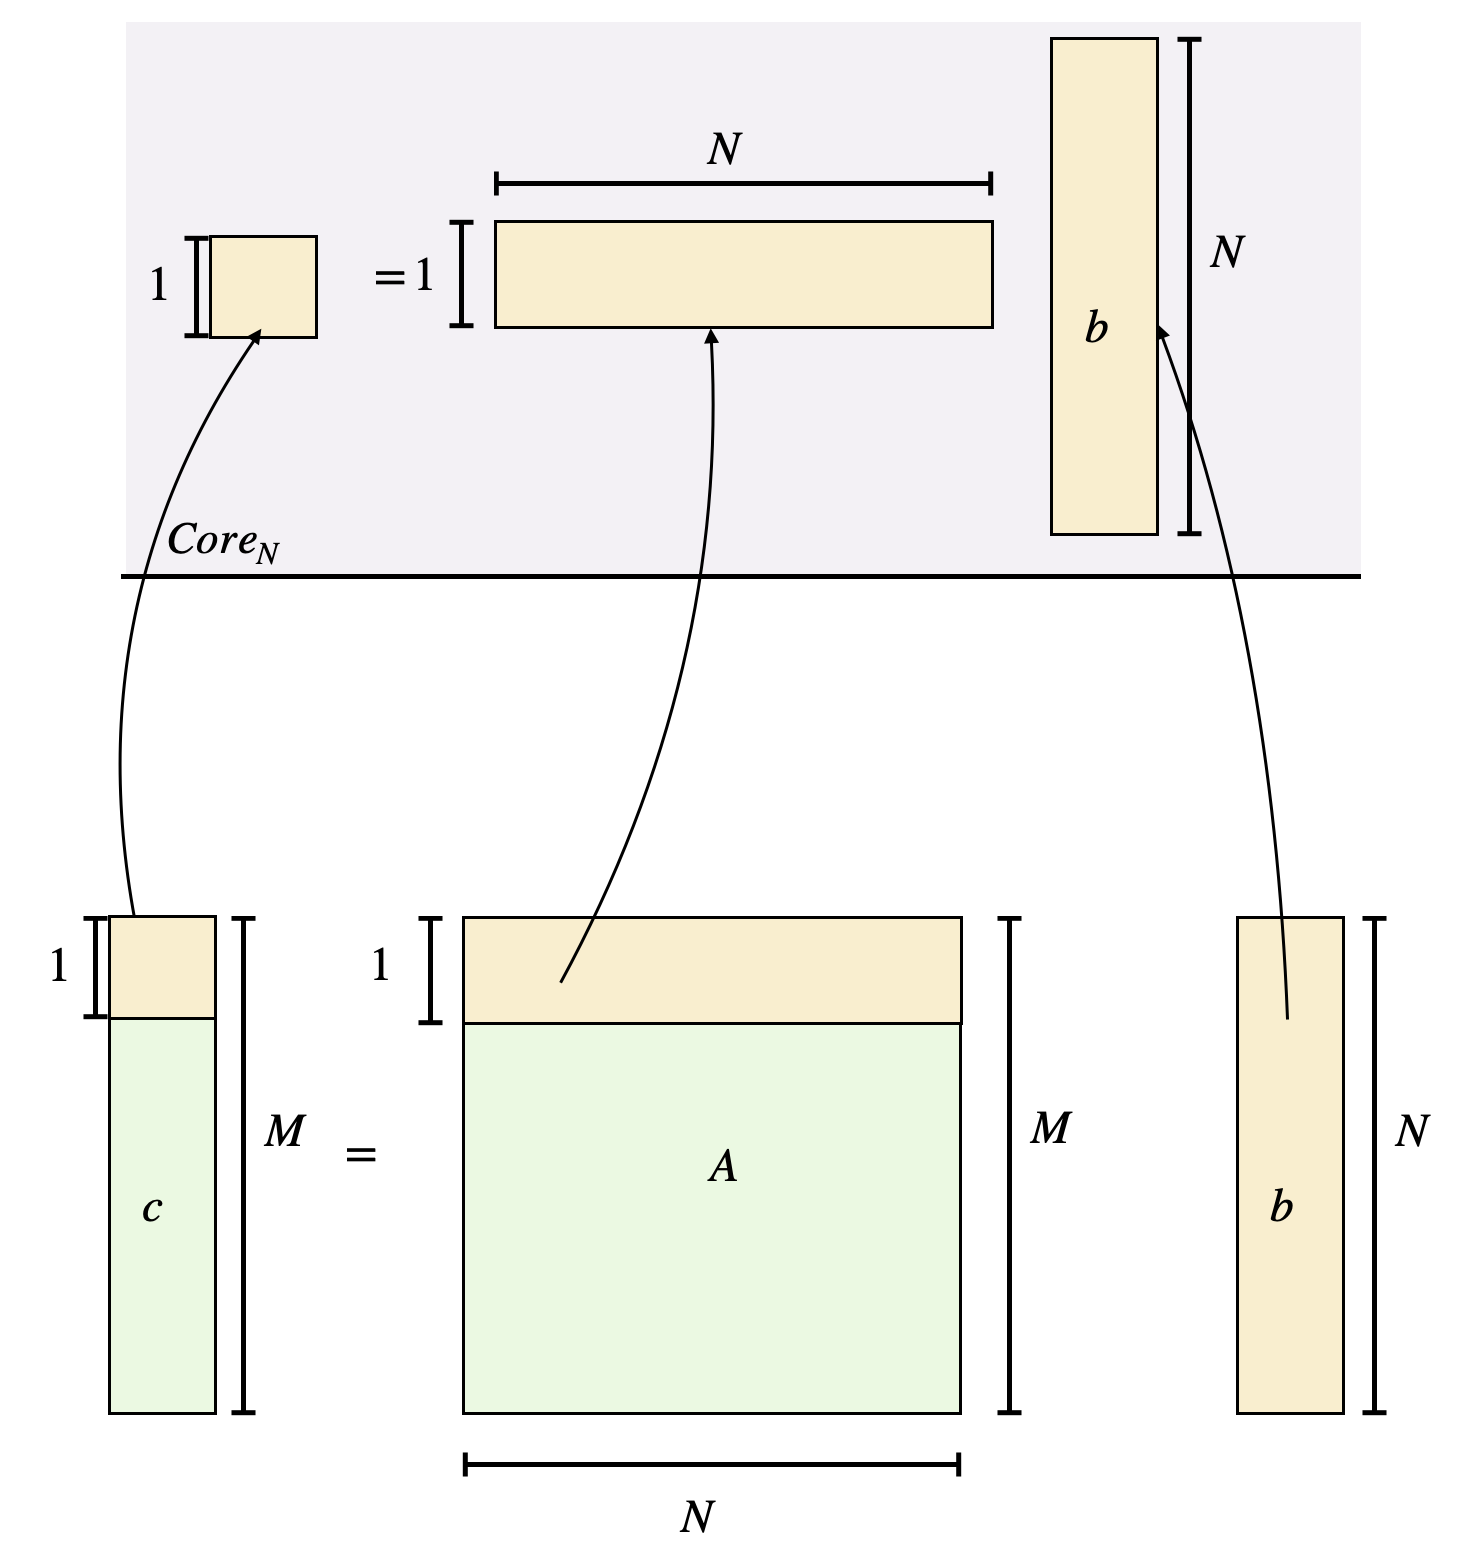
\includegraphics[width=15cm]{../assets/mtv/row_major/block_diagram.png} %
\end{figure}

\clearpage
\section{Performance Plots and Speedup Summary For Column-Major}

\begin{figure}[htb]
    \centering
    \caption*{Performance measurements of ?gemv implementations}
    \subfloat[\centering Single-Precision]{{\includegraphics[width=8cm]{../assets/mtv/col_major/float_GflopsVsSize.png} }}%
    \label{fig:mtv_col_Sgflop220}
    \qquad
    \subfloat[\centering Double-Precision]{{\includegraphics[width=8cm]{../assets/mtv/col_major/double_GflopsVsSize.png} }}%
    \label{fig:mtv_col_Dgflop220}
\end{figure}

\begin{figure}[htb]
    \centering
    \caption*{Sorted performance measurements of ?gemv implementations}
    \subfloat[\centering Single-Precision]{{\includegraphics[width=8cm]{../assets/mtv/col_major/float_GflopsVsSize_per.png} }}%
    \label{fig:mtv_col_Sgflop_per220}
    \qquad
    \subfloat[\centering Double-Precision]{{\includegraphics[width=8cm]{../assets/mtv/col_major/double_GflopsVsSize_per.png} }}%
    \label{fig:mtv_col_Dgflop_per220}
\end{figure}

\begin{figure}[htb]
    \centering
    \caption*{Comparison of the Boost.uBLAS.Tensor ?gemv implementation}
    \subfloat[\centering Single-Precision]{{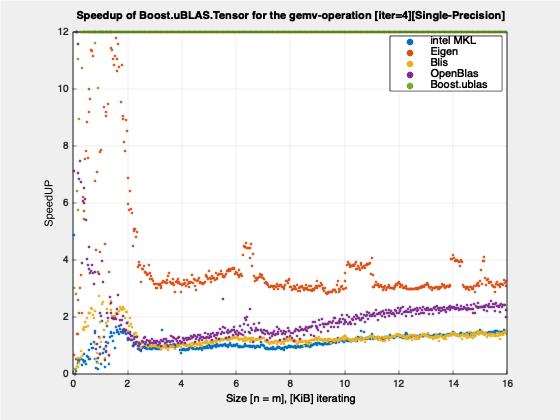
\includegraphics[width=8cm]{../assets/mtv/col_major/float_Speedup.png} }}%
    \label{fig:mtv_col_Sspeedup220}
    \qquad
    \subfloat[\centering Double-Precision]{{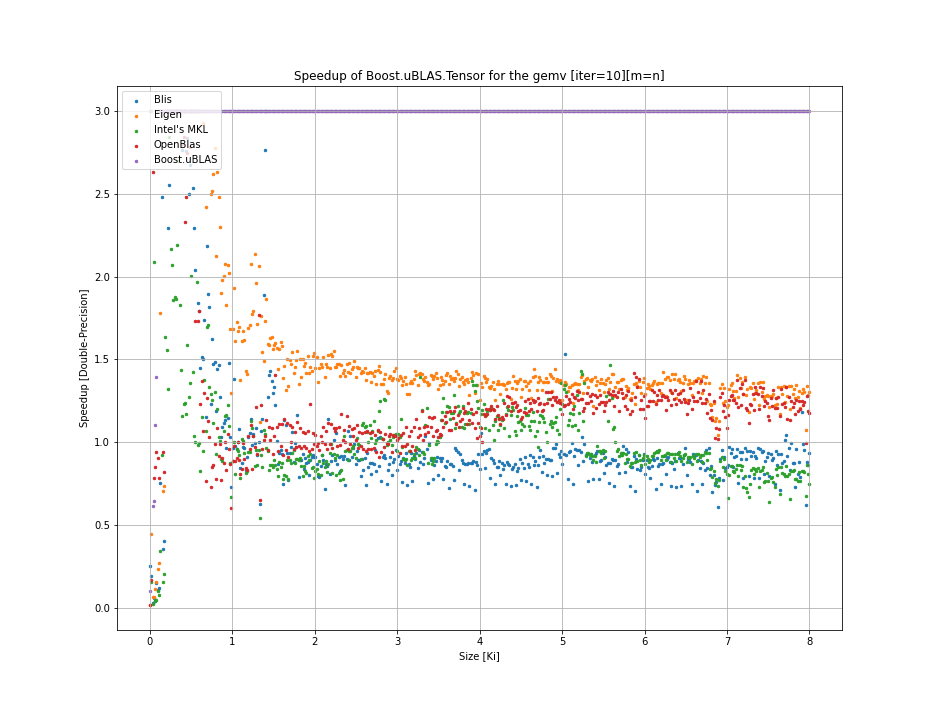
\includegraphics[width=8cm]{../assets/mtv/col_major/double_Speedup.png} }}%
    \label{fig:mtv_col_Dspeedup220}
\end{figure}

\begin{figure}[htb]
    \centering
    \caption*{Comparison of the Boost.uBLAS.Tensor ?gemv implementation [semilogy]}
    \subfloat[\centering Single-Precision]{{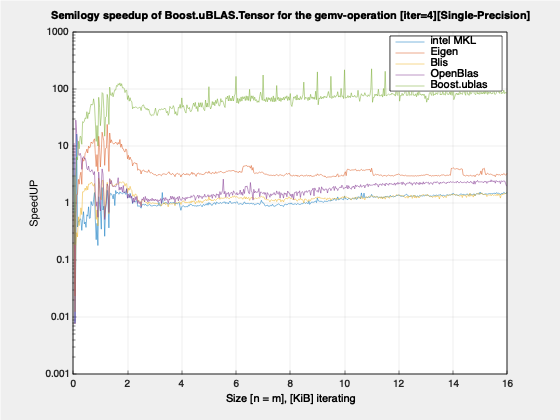
\includegraphics[width=8cm]{../assets/mtv/col_major/float_Speedup_log10.png} }}%
    \label{fig:mtv_col_Sspeedup_log10220}
    \qquad
    \subfloat[\centering Double-Precision]{{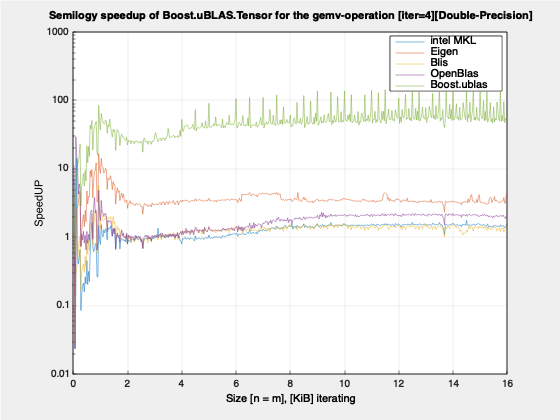
\includegraphics[width=8cm]{../assets/mtv/col_major/double_Speedup_log10.png} }}%
    \label{fig:mtv_col_Dspeedup_log10220}
\end{figure}

\begin{figure}[htb]
    \centering
    \caption*{Comparison of the Boost.uBLAS.Tensor ?gemv implementation [sorted]}
    \subfloat[\centering Single-Precision]{{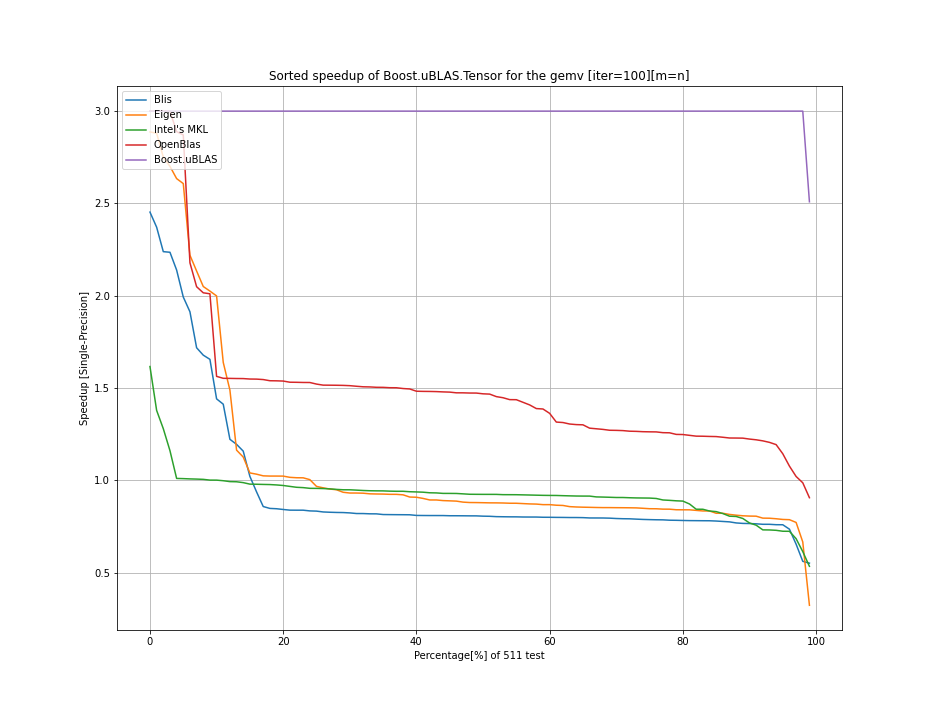
\includegraphics[width=8cm]{../assets/mtv/col_major/float_Speedup_per.png} }}%
    \label{fig:mtv_col_Sspeedup_per220}
    \qquad
    \subfloat[\centering Double-Precision]{{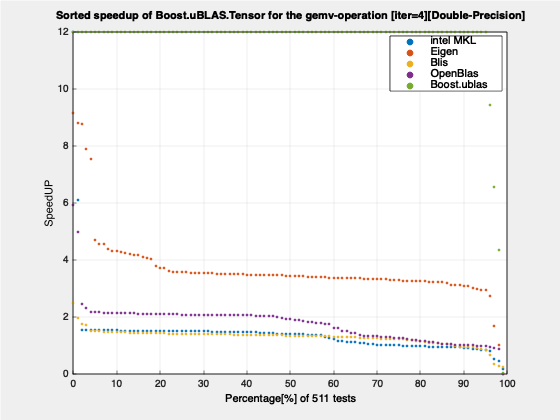
\includegraphics[width=8cm]{../assets/mtv/col_major/double_Speedup_per.png} }}%
    \label{fig:mtv_col_Dspeedup_per220}
\end{figure}

\begin{table}[ht]
    \centering
    \caption{Speedup Summary For Single-Precision}
    \begin{tabular}{|l|c|c|}
        \hline
        \textbf{Implementation} & \textbf{Speedup $\geq$ 1 [\%]} & \textbf{Speedup $\geq$ 2 [\%]}\\
        \hline
        Boost.uBLAS & $97$ & $97$ \\
        \hline
        OpenBLAS    & $98$ & $38$ \\
        \hline
        Eigen       & $97$ & $97$ \\
        \hline
        Blis        & $98$ & $98$ \\
        \hline
        Intel's MKL & $61$ & $1$ \\
        \hline
    \end{tabular}
    
    \begin{tabular}{|l|c|c|}
        \hline
        \textbf{Implementation} & \textbf{Speed-down $\geq$ 1 [\%]} & \textbf{Speed-down $\geq$ 2 [\%]}\\
        \hline
        Boost.uBLAS & $0$ & $0$ \\
        \hline
        OpenBLAS    & $0$ & $0$ \\
        \hline
        Eigen       & $1$ & $1$ \\
        \hline
        Blis        & $7$ & $1$ \\
        \hline
        Intel's MKL & $37$ & $0$ \\
        \hline
    \end{tabular}
    
    \vspace*{1 cm}

    \centering
    \caption{Speedup Summary For Double-Precision}
    \begin{tabular}{|l|c|c|}
        \hline
        \textbf{Implementation} & \textbf{Speedup $\geq$ 1 [\%]} & \textbf{Speedup $\geq$ 2 [\%]}\\
        \hline
        Boost.uBLAS & $98$ & $98$ \\
        \hline
        OpenBLAS    & $92$ & $47$ \\
        \hline
        Eigen       & $98$ & $96$ \\
        \hline
        Blis        & $87$ & $0$ \\
        \hline
        Intel's MKL & $76$ & $1$ \\
        \hline
    \end{tabular}
    
    \begin{tabular}{|l|c|c|}
        \hline
        \textbf{Implementation} & \textbf{Speed-down $\geq$ 1 [\%]} & \textbf{Speed-down $\geq$ 2 [\%]}\\
        \hline
        Boost.uBLAS & $0$ & $0$ \\
        \hline
        OpenBLAS    & $6$ & $0$ \\
        \hline
        Eigen       & $0$ & $0$ \\
        \hline
        Blis        & $11$ & $2$ \\
        \hline
        Intel's MKL & $22$ & $1$ \\
        \hline
    \end{tabular}
\end{table}

\clearpage
\section{Performance Metrics For Column-Major}

\subsection*{Range[Start: $32$, End: $16382$, Step: $32$]}

\begin{table}[ht]
    \centering
    \caption{GFLOPS For Single-Precision}
    \begin{tabular}{|l|c|c|}
        \hline
        \textbf{Implementation} & \textbf{Max} & \textbf{Average}\\
        \hline
        Boost.uBLAS.Tensor  & $63.1299$& $16.3994$ \\
        \hline
        Boost.uBLAS         & $1.04371$& $0.275396$ \\
        \hline
        Intel's MKL         & $82.2283$& $15.6702$ \\
        \hline
        OpenBLAS            & $31.4436$& $9.49543$ \\
        \hline
        Blis                & $28.142$& $12.4837$ \\
        \hline
        Eigen               & $7.59804$& $4.15489$ \\
        \hline
    \end{tabular}

    \vspace*{1 cm}

    \centering
    \caption{GFLOPS For Double-Precision}
    \begin{tabular}{|l|c|c|}
        \hline
        \textbf{Implementation} & \textbf{Max} & \textbf{Average}\\
        \hline
        Boost.uBLAS.Tensor  & $37.9093$ & $7.66141$ \\
        \hline
        Boost.uBLAS         & $0.585254$ & $0.184873$ \\
        \hline
        Intel's MKL         & $46.0515$ & $6.78875$ \\
        \hline
        OpenBLAS            & $12.3714$ & $4.69513$ \\
        \hline
        Blis                & $14.4262$ & $5.90106$ \\
        \hline
        Eigen               & $5.1347$ & $2.0504$ \\
        \hline
    \end{tabular}
\end{table}

\begin{table}[ht]
    \centering
    \caption{Utilization[\%] For Single-Precision}
    \begin{tabular}{|l|c|c|}
        \hline
        \textbf{Implementation} & \textbf{Max} & \textbf{Average}\\
        \hline
        Boost.uBLAS.Tensor  & $10.7218$& $2.78522$ \\
        \hline
        Boost.uBLAS         & $0.17726$& $0.0467724$ \\
        \hline
        Intel's MKL         & $13.9654$& $2.66137$ \\
        \hline
        OpenBLAS            & $5.34028$& $1.61268$ \\
        \hline
        Blis                & $4.77956$& $2.12019$ \\
        \hline
        Eigen               & $1.29043$& $0.705654$ \\
        \hline
    \end{tabular}

    \vspace*{1 cm}

    \centering
    \caption{Utilization[\%] For Double-Precision}
    \begin{tabular}{|l|c|c|}
        \hline
        \textbf{Implementation} & \textbf{Max} & \textbf{Average}\\
        \hline
        Boost.uBLAS.Tensor  & $12.8768$ & $2.60238$ \\
        \hline
        Boost.uBLAS         & $0.198795$ & $0.0627965$ \\
        \hline
        Intel's MKL         & $15.6425$ & $2.30596$ \\
        \hline
        OpenBLAS            & $4.20224$ & $1.59481$ \\
        \hline
        Blis                & $4.90021$ & $2.00443$ \\
        \hline
        Eigen               & $1.74412$ & $0.696469$ \\
        \hline
    \end{tabular}
\end{table}

\begin{table}[ht]
    \centering
    \caption{Speedup(Boost.uBLAS.Tensor) For Single-Precision}
    \begin{tabular}{|l|c|c|}
        \hline
        \textbf{Implementation} & \textbf{Max} & \textbf{Average}\\
        \hline
        Boost.uBLAS         & $60.4862$ & $59.5483$ \\
        \hline
        Intel's MKL         & $0.767739$ & $1.04653$ \\
        \hline
        OpenBLAS            & $2.00772$ & $1.72708$ \\
        \hline
        Blis                & $2.24326$ & $1.31366$ \\
        \hline
        Eigen               & $8.30871$ & $3.947$ \\
        \hline
    \end{tabular}

    \vspace*{1 cm}

    \centering
    \caption{Speedup(Boost.uBLAS.Tensor) For Double-Precision}
    \begin{tabular}{|l|c|c|}
        \hline
        \textbf{Implementation} & \textbf{Max} & \textbf{Average}\\
        \hline
        Boost.uBLAS         & $64.7741$ & $41.4415$ \\
        \hline
        Intel's MKL         & $0.823193$ & $1.12854$ \\
        \hline
        OpenBLAS            & $3.06427$ & $1.63178$ \\
        \hline
        Blis                & $2.6278$ & $1.29831$ \\
        \hline
        Eigen               & $7.38297$ & $3.73654$ \\
        \hline
    \end{tabular}
\end{table}

\clearpage
\section{Performance Plots and Speedup Summary For Row-Major}

\begin{figure}[htb]
    \centering
    \caption*{Performance measurements of ?gemv implementations}
    \subfloat[\centering Single-Precision]{{\includegraphics[width=8cm]{../assets/mtv/row_major/float_GflopsVsSize.png} }}%
    \label{fig:mtv_row_Sgflop220}
    \qquad
    \subfloat[\centering Double-Precision]{{\includegraphics[width=8cm]{../assets/mtv/row_major/double_GflopsVsSize.png} }}%
    \label{fig:mtv_row_Dgflop220}
\end{figure}

\begin{figure}[htb]
    \centering
    \caption*{Sorted performance measurements of ?gemv implementations}
    \subfloat[\centering Single-Precision]{{\includegraphics[width=8cm]{../assets/mtv/row_major/float_GflopsVsSize_per.png} }}%
    \label{fig:mtv_row_Sgflop_per220}
    \qquad
    \subfloat[\centering Double-Precision]{{\includegraphics[width=8cm]{../assets/mtv/row_major/double_GflopsVsSize_per.png} }}%
    \label{fig:mtv_row_Dgflop_per220}
\end{figure}

\begin{figure}[htb]
    \centering
    \caption*{Comparison of the Boost.uBLAS.Tensor ?gemv implementation}
    \subfloat[\centering Single-Precision]{{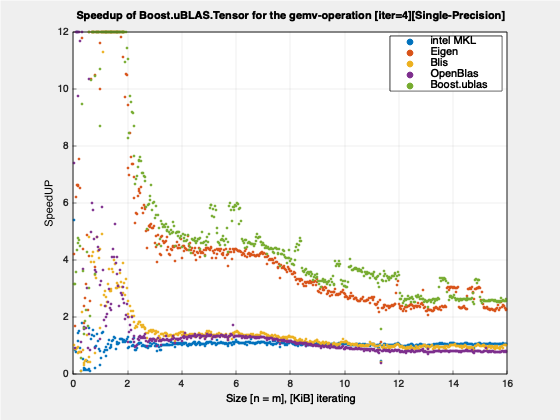
\includegraphics[width=8cm]{../assets/mtv/row_major/float_Speedup.png} }}%
    \label{fig:mtv_row_Sspeedup220}
    \qquad
    \subfloat[\centering Double-Precision]{{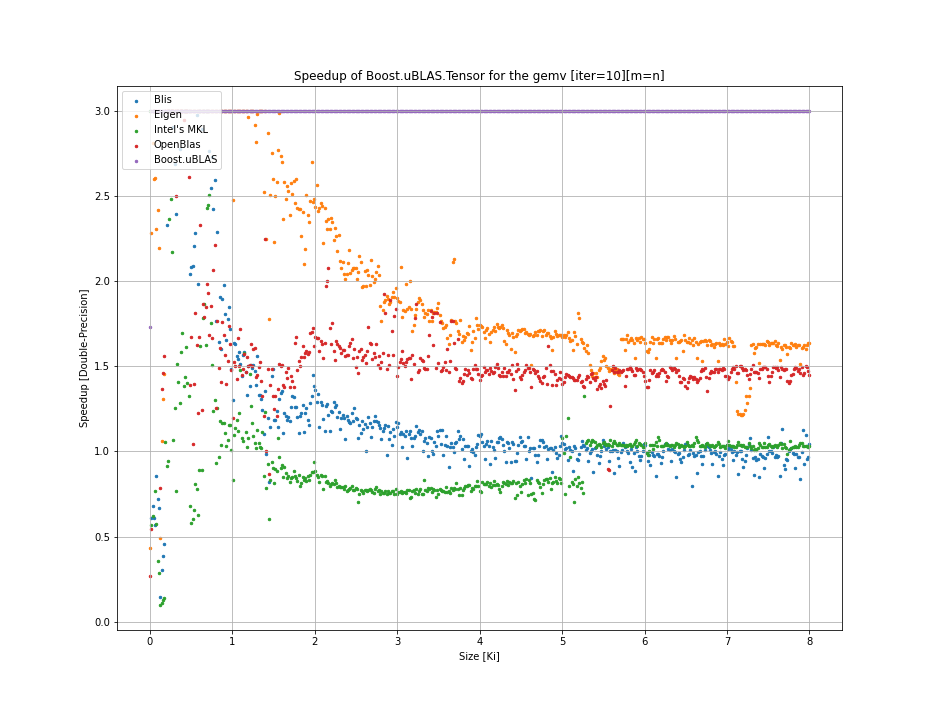
\includegraphics[width=8cm]{../assets/mtv/row_major/double_Speedup.png} }}%
    \label{fig:mtv_row_Dspeedup220}
\end{figure}

\begin{figure}[htb]
    \centering
    \caption*{Comparison of the Boost.uBLAS.Tensor ?gemv implementation [semilogy]}
    \subfloat[\centering Single-Precision]{{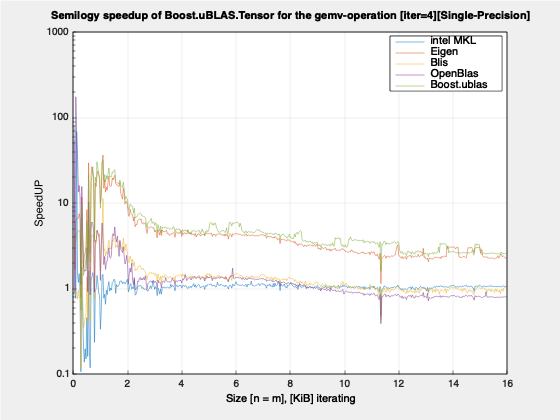
\includegraphics[width=8cm]{../assets/mtv/row_major/float_Speedup_log10.png} }}%
    \label{fig:mtv_row_Sspeedup_log10220}
    \qquad
    \subfloat[\centering Double-Precision]{{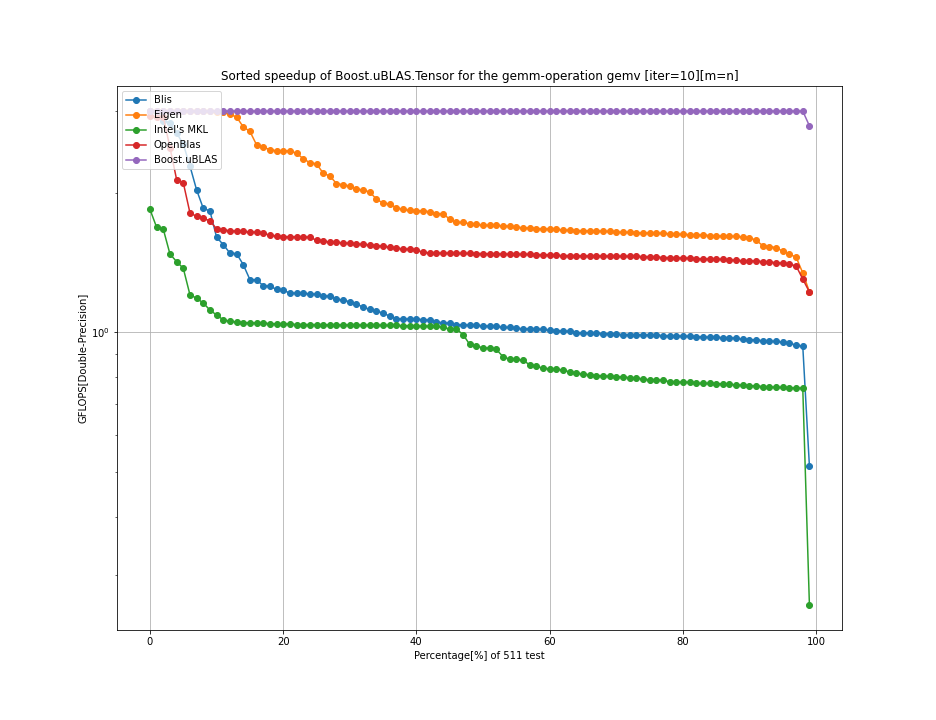
\includegraphics[width=8cm]{../assets/mtv/row_major/double_Speedup_log10.png} }}%
    \label{fig:mtv_row_Dspeedup_log10220}
\end{figure}

\begin{figure}[htb]
    \centering
    \caption*{Comparison of the Boost.uBLAS.Tensor ?gemv implementation [sorted]}
    \subfloat[\centering Single-Precision]{{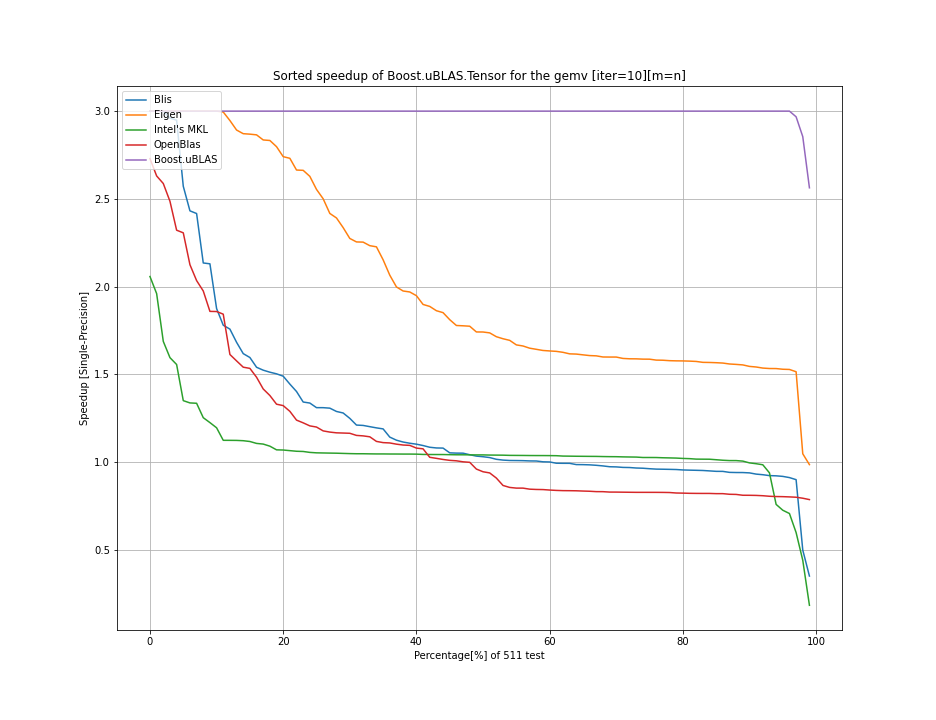
\includegraphics[width=8cm]{../assets/mtv/row_major/float_Speedup_per.png} }}%
    \label{fig:mtv_row_Sspeedup_per220}
    \qquad
    \subfloat[\centering Double-Precision]{{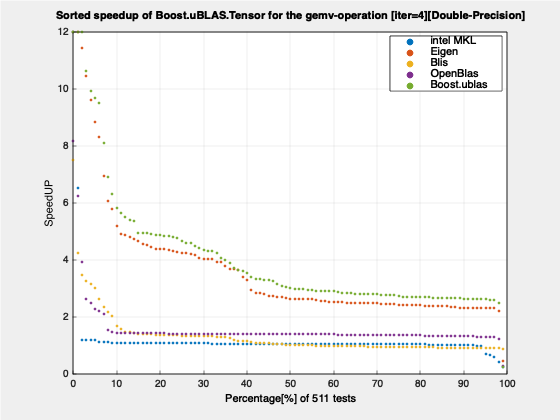
\includegraphics[width=8cm]{../assets/mtv/row_major/double_Speedup_per.png} }}%
    \label{fig:mtv_row_Dspeedup_per220}
\end{figure}

\begin{table}[ht]
    \centering
    \caption{Speedup Summary For Single-Precision}
    \begin{tabular}{|l|c|c|}
        \hline
        \textbf{Implementation} & \textbf{Speedup $\geq$ 1 [\%]} & \textbf{Speedup $\geq$ 2 [\%]}\\
        \hline
        Boost.uBLAS & $98$ & $98$ \\
        \hline
        OpenBLAS    & $56$ & $10$ \\
        \hline
        Eigen       & $98$ & $97$ \\
        \hline
        Blis        & $73$ & $9$ \\
        \hline
        Intel's MKL & $88$ & $1$ \\
        \hline
    \end{tabular}
    
    \begin{tabular}{|l|c|c|}
        \hline
        \textbf{Implementation} & \textbf{Speed-down $\geq$ 1 [\%]} & \textbf{Speed-down $\geq$ 2 [\%]}\\
        \hline
        Boost.uBLAS & $0$ & $0$ \\
        \hline
        OpenBLAS    & $42$ & $0$ \\
        \hline
        Eigen       & $0$ & $0$ \\
        \hline
        Blis        & $25$ & $0$ \\
        \hline
        Intel's MKL & $10$ & $0$ \\
        \hline
    \end{tabular}
    
    \vspace*{1 cm}

    \centering
    \caption{Speedup Summary For Double-Precision}
    \begin{tabular}{|l|c|c|}
        \hline
        \textbf{Implementation} & \textbf{Speedup $\geq$ 1 [\%]} & \textbf{Speedup $\geq$ 2 [\%]}\\
        \hline
        Boost.uBLAS & $98$ & $98$ \\
        \hline
        OpenBLAS    & $98$ & $7$ \\
        \hline
        Eigen       & $98$ & $98$ \\
        \hline
        Blis        & $59$ & $9$ \\
        \hline
        Intel's MKL & $92$ & $1$ \\
        \hline
    \end{tabular}
    
    \begin{tabular}{|l|c|c|}
        \hline
        \textbf{Implementation} & \textbf{Speed-down $\geq$ 1 [\%]} & \textbf{Speed-down $\geq$ 2 [\%]}\\
        \hline
        Boost.uBLAS & $0$ & $0$ \\
        \hline
        OpenBLAS    & $0$ & $0$ \\
        \hline
        Eigen       & $0$ & $0$ \\
        \hline
        Blis        & $39$ & $0$ \\
        \hline
        Intel's MKL & $6$ & $1$ \\
        \hline
    \end{tabular}
\end{table}

\clearpage
\section{Performance Metrics For Row-Major}

\subsection*{Range[Start: $32$, End: $16382$, Step: $32$]}

\begin{table}[ht]
    \centering
    \caption{GFLOPS For Single-Precision}
    \begin{tabular}{|l|c|c|}
        \hline
        \textbf{Implementation} & \textbf{Max} & \textbf{Average}\\
        \hline
        Boost.uBLAS.Tensor  & $114.495$& $19.4496$ \\
        \hline
        Boost.uBLAS         & $4.86818$& $3.62716$ \\
        \hline
        Intel's MKL         & $103.86$& $19.2955$ \\
        \hline
        OpenBLAS            & $39.0813$& $14.0183$ \\
        \hline
        Blis                & $28.5224$& $12.8971$ \\
        \hline
        Eigen               & $8.70003$& $4.11144$ \\
        \hline
    \end{tabular}

    \vspace*{1 cm}

    \centering
    \caption{GFLOPS For Double-Precision}
    \begin{tabular}{|l|c|c|}
        \hline
        \textbf{Implementation} & \textbf{Max} & \textbf{Average}\\
        \hline
        Boost.uBLAS.Tensor  & $48.6174$& $8.13646$ \\
        \hline
        Boost.uBLAS         & $2.19048$& $1.82291$ \\
        \hline
        Intel's MKL         & $51.6863$& $8.51818$ \\
        \hline
        OpenBLAS            & $18.6354$& $5.19158$ \\
        \hline
        Blis                & $14.9491$& $6.06728$ \\
        \hline
        Eigen               & $6.28753$& $2.04718$ \\
        \hline
    \end{tabular}
\end{table}

\begin{table}[ht]
    \centering
    \caption{Utilization[\%] For Single-Precision}
    \begin{tabular}{|l|c|c|}
        \hline
        \textbf{Implementation} & \textbf{Max} & \textbf{Average}\\
        \hline
        Boost.uBLAS.Tensor  & $19.4456$& $3.30327$ \\
        \hline
        Boost.uBLAS         & $0.826797$& $0.616026$ \\
        \hline
        Intel's MKL         & $17.6393$& $3.27708$ \\
        \hline
        OpenBLAS            & $6.63744$& $2.38082$ \\
        \hline
        Blis                & $4.84416$& $2.1904$ \\
        \hline
        Eigen               & $1.47759$& $0.698275$ \\
        \hline
    \end{tabular}

    \vspace*{1 cm}

    \centering
    \caption{Utilization[\%] For Double-Precision}
    \begin{tabular}{|l|c|c|}
        \hline
        \textbf{Implementation} & \textbf{Max} & \textbf{Average}\\
        \hline
        Boost.uBLAS.Tensor  & $16.5141$& $2.76374$ \\
        \hline
        Boost.uBLAS         & $0.744048$& $0.619195$ \\
        \hline
        Intel's MKL         & $17.5565$& $2.89341$ \\
        \hline
        OpenBLAS            & $6.32996$& $1.76344$ \\
        \hline
        Blis                & $5.07782$& $2.0609$ \\
        \hline
        Eigen               & $2.13571$& $0.695374$ \\
        \hline
    \end{tabular}
\end{table}

\begin{table}[ht]
    \centering
    \caption{Speedup(Boost.uBLAS.Tensor) For Single-Precision}
    \begin{tabular}{|l|c|c|}
        \hline
        \textbf{Implementation} & \textbf{Max} & \textbf{Average}\\
        \hline
        Boost.uBLAS         & $23.5192$& $5.36222$ \\
        \hline
        Intel's MKL         & $1.1024$& $1.00799$ \\
        \hline
        OpenBLAS            & $2.92968$& $1.38745$ \\
        \hline
        Blis                & $4.01423$& $1.50807$ \\
        \hline
        Eigen               & $13.1604$& $4.73061$ \\
        \hline
    \end{tabular}

    \vspace*{1 cm}

    \centering
    \caption{Speedup(Boost.uBLAS.Tensor) For Double-Precision}
    \begin{tabular}{|l|c|c|}
        \hline
        \textbf{Implementation} & \textbf{Max} & \textbf{Average}\\
        \hline
        Boost.uBLAS         & $22.1949$& $4.46344$ \\
        \hline
        Intel's MKL         & $0.940624$& $0.955187$ \\
        \hline
        OpenBLAS            & $2.60887$& $1.56724$ \\
        \hline
        Blis                & $3.25219$& $1.34104$ \\
        \hline
        Eigen               & $7.73235$& $3.97447$ \\
        \hline
    \end{tabular}
\end{table}